\documentclass[tikz]{standalone}
\usepackage{import}
\usepackage{tkz-euclide}

\begin{document}
    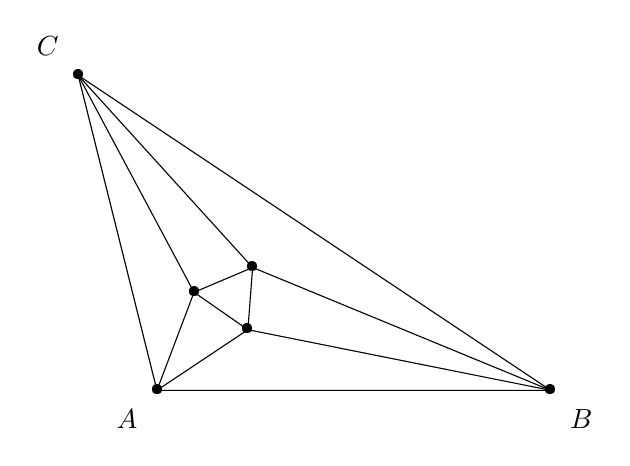
\begin{tikzpicture}
        \coordinate (A) at (0, 0);
        \coordinate (B) at (5, 0);
        \coordinate (C) at (-1, 4);
        
        \draw (A) -- (B) -- (C) -- (A);
        
        \coordinate (D) at (0.471, 1.245);
        \coordinate (E) at (1.155, 0.77);
        \coordinate (F) at (1.215, 1.56);
        
        \draw (D) -- (E) -- (F) -- (D);
        \draw (A) -- (D);
        \draw (A) -- (E);
        \draw (B) -- (E);
        \draw (B) -- (F);
        \draw (C) -- (F);
        \draw (C) -- (D);
        
        \node[black] at (A) {\textbullet};
        \node[black] at (B) {\textbullet};
        \node[black] at (C) {\textbullet};
        \node[black] at (D) {\textbullet};
        \node[black] at (E) {\textbullet};
        \node[black] at (F) {\textbullet};
        
        \draw (A) node[label={[label distance=0cm]225:$A$}]{}
              (B) node[label={[label distance=0cm]315:$B$}]{}
              (C) node[label={[label distance=0cm]135:$C$}]{};
    \end{tikzpicture}
\end{document}
